\subsection{Caractéristiques de la Programmation Orienté Objet}

\newcommand{\bizProcessExemple}[0]{
  \begin{enumerate}
    \item créer un nouveau salarié dans la base de données
    \item ajouter la salarié dans l'équipe de son manager
    \item notifier par email les membres de l'équipe de l'arrivée du nouveau membre
  \end{enumerate}
}

\ifbook{

  \paragraph{} La paradigme de la programmation orienté objet se retrouve dans  plusieurs
  problématiques liées au \textbf{Middleware}, il est important d'expliciter quelques unes de ses
  caractéristiques.

  \subsection{Programmation impérative}

  \paragraph{} La paradigme de la programmation orienté objet se retrouve dans  plusieurs
  problématiques liées au \textbf{Middleware}, il est important d'expliciter quelques unes de ses
  caractéristiques.

  \paragraph{} En premier lieu, il faut savoir que la programmation orienté object se définit
  essentiellement par sa distinction avec la programmation \textbf{procédurale} ou
  \textbf{impérative}. Dans ce style de programmation, on effectue les traitements les uns à la suite
  des autres, en regroupant le code commun dans des fonctions.

  \paragraph{} Prenons l'exemple de traitement procédurale:

  \bizProcessExemple

  \paragraph{} Une approche impérative consisterait ici à réaliser un programme réalisant chacune de
  ces actions, dans l'ordres. C'est une approche tout à fait valide et elle ne pose pas, en soi, de
  problème.

  \subsection{Approche par "objet"}

  \paragraph{} Néanmoins, la programmation orienté objet propose une approche, qui apporte de nombreux
  avantages. Cette approche consiste à ne plus se concentrer sur la séquence de traitement à réaliser,
  mais plutôt sur les données utilisées.

  \paragraph{} En effet, le but du jeu ici est d'\textbf{encapsuler} les données dans des objets, et
  ne le laisse le reste du programme interagir avec ces données que par le biais des fonctions
  qu'elles proposent. Ces fonctiones se nomment en fait désormais des \textbf{méthodes}.

  \paragraph{} L'objectif de ceci est de \textbf{masquer} la nature réelle des données, et de
  n'exposer que les traitements disponibles autour de ces données. Ainsi, si la nature des données ou
  même des détails d'implémentations des traitements proposés venaient à changer, ces modifications
  seront transparente pour le reste du programme.
}

\ifslide {
  \subsection{Programmation impérative versus programmation orienté objet}
  \begin{frame}
    \begin{block}{Ajout d'un nouvel employé}
      \bizProcessExemple
    \end{block}
    \begin{center}
      
\includegraphics[scale=0.30]{img/biz-process-banner.png}
    \end{center}
  \end{frame}
}

\ifbook{

  \paragraph{} Illustrons ce point en reprenant notre exemple précédent. Pour implémenter notre
  processus métier - l'ajout d'un nouveau employé dans une équipe, nous allons désormais définir
  plusieurs \textbf{objet}.

  \paragraph{} Le premier objet sera l'objet salarié. Ce dernier résultura de la création du salarié
  dans la base de données de l'entreprise, et il regroupe l'ensemble des données relatives à un
  employé. L'accès à la base de données des salariés sera aussi un objet.

  \paragraph{} Le second objet sera en fait une collection de salarié que forme son équipe. Pour
  réaliser le second point de notre traitement, il suffira donc d'ajouter le salarié créée juste avant
  à la liste des salariés composant l'équipe.

  \paragraph{} Un autre objet sera en charge de l'envoi des mails, et sera donc utilisé pour notifier
  les différents membres de l'équipe de l'arrivée du nouveau membre de l'équipe.
}

\ifslide{
  \begin{frame}
    \begin{center}
      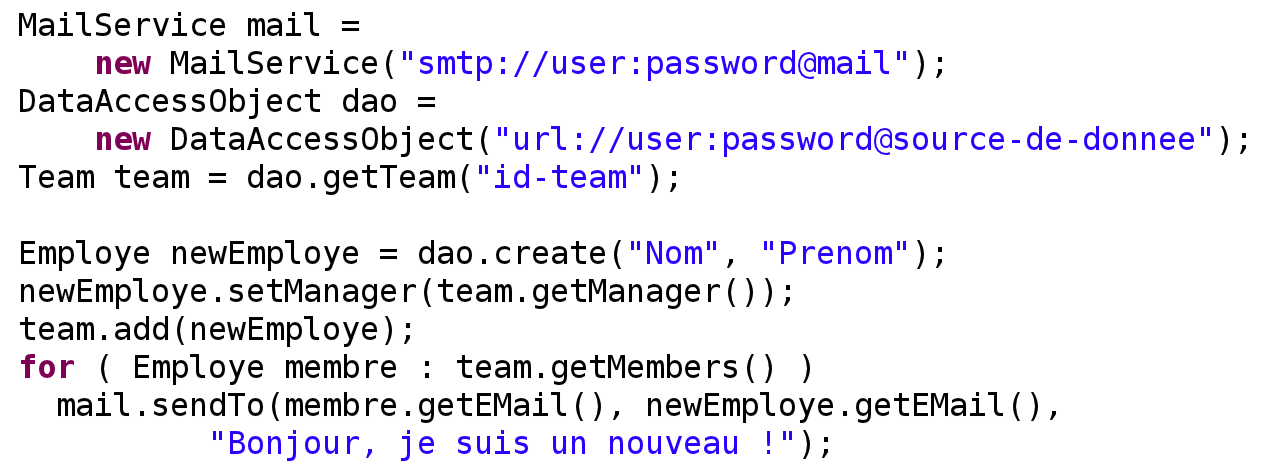
\includegraphics[scale=0.25]{img/biz-process-code-sample.png}
    \end{center}
  \end{frame}
}

\ifbook{

  \begin{figure}[h]
    \begin{center}
      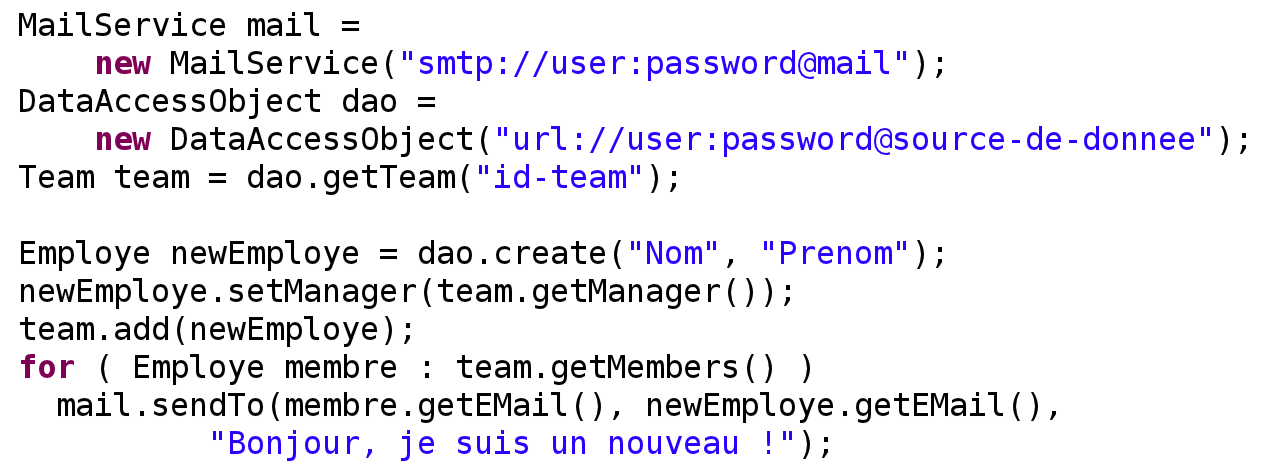
\includegraphics[scale=0.35]{img/biz-process-code-sample.png}
      \caption{Exemple de code orienté objet}
      \label{biz-process-code}
    \end{center}
  \end{figure}

  \paragraph{} Comme l'illustre l'extrait de code \ref{biz-process-code} (page
  \pageref{biz-process-code}, ce style de programmation qu'est la  programmation orienté objet
  permet d'obtenir un code très simple et lisible, mais surtout facilement réutilisable. Par
  exemple, l'objet DataAccessObject regroupe tout le code nécessaire pour se connecter à la base de
  données. Il suffit de réutiliser cet objet, ailleurs dans le code du programme si l'on souhaite
  effectuer des opérations avec la base de données.

  \paragraph{} Un autre avantage immédiat de cette approche est de pouvoir concevoir aisément des
  objets "métiers" décrivant de manière isolé et unitaire, les différents traitements spécifique au
  métier de l'entreprise ou l'organisation. Les différents applications pourront ensuite aisément
  s'appuyer sur ces bibliothèques d'objets pour réaliser les différents traitements qui leur sont
  spécifiques.
}

%- dessin "application" => "pile, gestion de threads, cache, ...", puis vers le modèle java/jee de container
%- évoqué la problématique du packaging et de la réutilisation de code, probablématique de gestion de version aussi

% expliciter/décrire le besoin, dans la conception d'un IT, de découper son "business" en module,
% d'avoir est du code partagé (des Jars) mais aussi des applicatifs qui utilisent les mêmes briques,
% les mêmes services, etc...
